\section{Reducibility, Periodicity, and Transience in a Countable State Space}
\label{sec:A.3}

A Markov chain taking values on a countable state space $E$ is ergodic if it is irreducible,
aperiodic, and positive recurrent.  We now review these concepts in the context of countable state
space and then generalize them to general state space.

\begin{definition}[Irreducible Markov Chain]
\label{def:A.13}
A Markov chain is irreducible if all states intercommunicate.  That is, if for all $i, j \in E$
there is $n \geq 0$ such that
\[
  \Prob(X_n = i \mid X_0 = j) > 0.
\]
\end{definition}

\begin{definition}[Recurrent Markov Chain]
\label{def:A.14}
A Markov chain is recurrent if, for all $i \in E$,
\[
  \Prob(\mathbb{X} \text{ visits } i \text{ eventually} \mid X_0 = i) = 1.
\]
\end{definition}

\begin{definition}[Transient Markov Chain]
\label{def:A.15}
A Markov chain is transient if, for all $i \in E$,
\[
  \Prob(\mathbb{X} \text{ visits } i \text{ eventually} \mid X_0 = i) = 0.
\]
\end{definition}

\begin{definition}[Positive Recurrent Markov Chain]
\label{def:A.16}
A Markov chain is positive recurrent if $\Expect[T_{ii}] < \infty$ for all $i \in E$, where
$T_{ii}$ is the time of the first return to state $i$.
\end{definition}

\begin{definition}[Aperiodic Markov Chain]
\label{def:A.17}
A Markov chain is aperiodic if all states have period~$1$.  The period of state $i \in E$ is
defined as
\[
  d(i) := \gcd\{n > 0 : p^n(i, i) > 0\},
\]
where $\gcd$ stands for greatest common divisor.
\end{definition}

\begin{example}[Periodicity]
\label{ex:A.18}
For this chain
\begin{center}
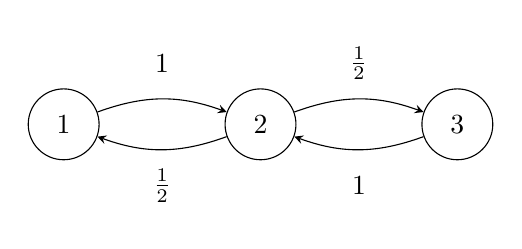
\begin{tikzpicture}[
    node distance=2.5cm,
    every node/.style={circle, draw, minimum size=0.9cm},
    >=stealth
  ]
  \node (1) {$1$};
  \node (2) [right of=1] {$2$};
  \node (3) [right of=2] {$3$};
  \draw[->] (1) to[bend left=20] node[draw=none,above] {$1$} (2);
  \draw[->] (2) to[bend left=20] node[draw=none,above] {$\frac{1}{2}$} (3);
  \draw[->] (2) to[bend left=20] node[draw=none,below] {$\frac{1}{2}$} (1);
  \draw[->] (3) to[bend left=20] node[draw=none,below] {$1$} (2);
\end{tikzpicture}
\end{center}
we can return to state~$1$ after $2, 4, 6, \ldots$ steps.  Hence, state~$1$ has period~$2$.
\end{example}

\begin{example}[Aperiodic State]
\label{ex:A.19}
For this chain
\begin{center}
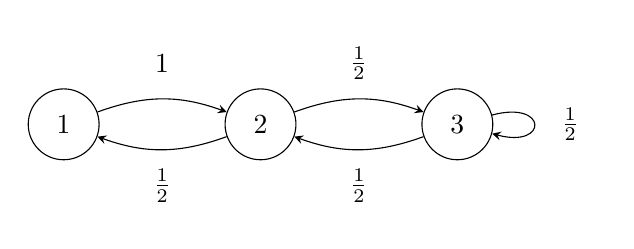
\begin{tikzpicture}[
    node distance=2.5cm,
    every node/.style={circle, draw, minimum size=0.9cm},
    >=stealth
  ]
  \node (1) {$1$};
  \node (2) [right of=1] {$2$};
  \node (3) [right of=2] {$3$};
  \draw[->] (1) to[bend left=20] node[draw=none,above] {$1$} (2);
  \draw[->] (2) to[bend left=20] node[draw=none,above] {$\frac{1}{2}$} (3);
  \draw[->] (2) to[bend left=20] node[draw=none,below] {$\frac{1}{2}$} (1);
  \draw[->] (3) to[loop right] node[draw=none,right] {$\frac{1}{2}$} (3);
  \draw[->] (3) to[bend left=20] node[draw=none,below] {$\frac{1}{2}$} (2);
\end{tikzpicture}
\end{center}
we can return to state~$1$ after $2, 4, 6, 7, \ldots$ steps.  Hence, state~$1$ has period~$1$.
\end{example}

\begin{example}[Periodic Chain]
\label{ex:A.20}
This is a periodic chain:
\begin{center}
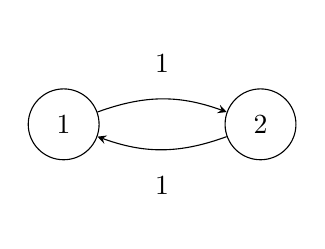
\begin{tikzpicture}[
    node distance=2.5cm,
    every node/.style={circle, draw, minimum size=0.9cm},
    >=stealth
  ]
  \node (1) {$1$};
  \node (2) [right of=1] {$2$};
  \draw[->] (1) to[bend left=20] node[draw=none,above] {$1$} (2);
  \draw[->] (2) to[bend left=20] node[draw=none,below] {$1$} (1);
\end{tikzpicture}
\end{center}
Note that
\[
  P = \begin{bmatrix} 0 & 1 \\ 1 & 0 \end{bmatrix}, \quad
  P^2 = \begin{bmatrix} 1 & 0 \\ 0 & 1 \end{bmatrix}, \quad
  P^3 = \begin{bmatrix} 0 & 1 \\ 1 & 0 \end{bmatrix}, \quad \ldots
\]
and so the transition probabilities do not converge as $n \to \infty$.  Also $P^n$ has some zero
entries for all $n \geq 1$.
\end{example}

\begin{remark}
\label{rem:A.21}
Recurrence and aperiodicity are chain properties.  If a Markov chain is irreducible, the whole
space is a communicating chain.  Therefore, if one state is recurrent, then the whole space is
recurrent (for irreducible chains).  Irreducibility ensures that the state space doesn't split into
subsets such that the chain cannot move from one subset to the others.  (Positive) recurrence
ensures that the chain eventually visits every subset of the state space of positive mass
(sufficiently often).  Periodicity causes the state space to split into subsets (cyclically moving
chains) which are visited by the chain in sequential order.
\end{remark}
